\chapter{The MultiRoute Family}
\label{chap:cornerstones}
\label{sect:multiroutes}
\begin{flushright}
 \textit{\textquotedblleft There is always a better strategy than the one you
have; \\ 
you just haven't thought of it yet\textquotedblright}\\
\textit{-- Sir Brian Pitman}
\end{flushright}


\ifpdf
    \graphicspath{{5-CornerMultipath/Chapter5Figs}{5-CornerMultipath/Chapter5Figs/PDF/}{5-CornerMultipath/Chapter5Figs/}}
\else
    \graphicspath{{5-CornerMultipath/Chapter5Figs/EPS/}{5-CornerMultipath/Chapter5Figs/}}
\fi

We now present the MultiRoute suite of congestion-aware inter-gateway routing protocols. But
first, we should define the path discovery strategy employed by MultiRoute
variants as it is identical and fundamental to all protocols. Then, we will
describe MultiRoute Monitoring Protocol (MMP) which is responsible for the
dissemination of congestion information throughout the network. While it differs
slightly from protocol to protocol, its essential basis stays unchanged within
each protocol. 

Next, we will follow RFC 1264 \cite{RFC1264} which describes the procedures for
creating and documenting standards on routing protocols. While this RFC has
been obsoleted for practical reason, the author still believes that some
aspects of the RFC can be used.


\section{Path Discovery}


Modern computer networks may offer many paths from any source to any
destination but current protocols only employ the shortest path or make use of
multiple paths of minimum cost if they exist. 

The first goal of any routing protocol is to discover the shortest path, while
a multipath protocol must also discover the possible alternative paths. We have
employed a technique similar to the one present in IGRP \cite{pat:IGRP}, which
allows a router to forward packets through paths whose length is less than the
product of the shortest path length and the variance factor. Since such an
approach may lead to routing loops\footnote{Routing onto paths which are
longer than the shortest path is known to lead to routing loops.}, we have
employed a slightly modified Relaxed
best path criterion \cite{OMP}.

\subsection{MultiRoute Path Construction (MRPC)}
\label{sect:MRPC}

MultiRoute's path construction algorithm relies heavily on Dijkstra's Shortest
Path algorithm \cite{DIJK}. However, the idea here is not only to discover the
shortest paths between any source-destination pair, but also find all the
available paths whether they are of equal length or within an acceptable
delta of the shortest path length. This is achieved through the use of two
parameters to the algorithm, the first represents the tolerable cost deviation
($\delta$) which we accept, the second being the maximal hop count deviation
(H). Both of these parameters are set by the network engineer, and should be
chosen carefully as they directly affect the latency versus throughput
trade-off.

The MRPC algorithm can be explained as a two phase algorithm. First, the
algorithm constructs a set of paths identical to OSPF, ie. the shortest paths,
each shortest path cost is then set as the reference cost. Second, considering
the
$\delta$ parameter, the algorithm now computes the potentially longer
alternative paths. Let the value $\alpha$ to be the shortest path from
some node \textit{A} on route to a destination node \textit{B}, and set $\beta$
as the length of the alternative path which passes through node \textit{C}. The
algorithm, then, visits the alternative path
possibilities, by checking whether $\beta \leq \alpha + \delta$, and if so it
adds this alternative path to the list of available paths. By the end of the
algorithm we are guaranteed to obtain a set of alternative paths whose lengths
are no longer than $\delta$ plus the shortest path length (See proof in
Section \ref{appdx:mrpc}).

\begin{figure}[htbp!]
\begin{center}
\begin{tikzpicture}[>=latex']
 \SetUpEdge[lw         = 1.5pt,
            color      = black]
            %labelcolor = black!30]
            %labelstyle = {draw,sloped}]
  \tikzset{node distance = 3cm}
  \GraphInit[vstyle=Normal]
\tikzset{EdgeStyle/.style={->}}
\tikzset{EdgeStyle/.append style = {bend left = 10}}
  \Vertex{1}


  \NOEA(1){2}
  \SOEA(1){8}
  \EA(2){3}
  \SO(3){4}
  \EA(4){5}
  \SO(4){7}
  \EA(7){6}

  \Edge[label=$0$](1)(2)
\Edge[label=$0$](1)(8)
  \Edge[label=$6$](2)(1)
  \Edge[label=$5$](8)(1)
  \Edge[label=$6$](2)(8)
 % \tikzset{EdgeStyle/.style={<->}} $\varepsilon$-property 
  \Edge[label=$5$](8)(2)
  \Edge[label=$6$](2)(3)
  \Edge[label=$4$](3)(2)
  \Edge[label=$6$](2)(4)
  \Edge[label=$7$](4)(2)
  %\tikzset{EdgeStyle/.style={<->,relative=false,in=0,out=60}}
  \Edge[label=$5$](8)(4)
  \Edge[label=$7$](4)(8)
  \Edge[label=$7$](4)(3)
  \Edge[label=$4$](3)(4)
  \Edge[label=$4$](3)(5)
  \Edge[label=$6$](5)(3)
  \Edge[label=$7$](4)(5)
  \Edge[label=$6$](5)(4)
  \Edge[label=$7$](4)(7)
    \Edge[label=$3$](7)(4)
  \Edge[label=$3$](7)(6)
  \Edge[label=$2$](6)(7)
  \Edge[label=$6$](5)(6)
  \Edge[label=$2$](6)(5)
\end{tikzpicture}
\end{center}

\centering
$\Big \Downarrow$

\begin{center}
\begin{tikzpicture}[>=latex']
 \SetUpEdge[lw         = 1.5pt,
            color      = black]
            %labelcolor = black!30]
            %labelstyle = {draw,sloped}]
  \tikzset{node distance = 3cm}
  \GraphInit[vstyle=Normal]
\tikzset{EdgeStyle/.style={->}}
\tikzset{EdgeStyle/.append style = {bend left = 10}}
  \Vertex{1}


  \NOEA(1){2}
  \SOEA(1){8}
  \EA(2){3}
  \SO(3){4}
  \EA(4){5}
  \SO(4){7}
  \EA(7){6}

  \Edge[label=$0$](1)(2)
\Edge[label=$0$](1)(8)


 % \tikzset{EdgeStyle/.style={<->}}

  \Edge[label=$6$](2)(3)



  %\tikzset{EdgeStyle/.style={<->,relative=false,in=0,out=60}}
  \Edge[label=$5$](8)(4)
  \Edge[label=$6$](2)(4)

  %\Edge[label=$4$](3)(4)
  \Edge[label=$4$](3)(5)

  \Edge[label=$7$](4)(5)

  \Edge[label=$7$](4)(7)

  \Edge[label=$3$](7)(6)

  \Edge[label=$6$](5)(6)

\end{tikzpicture}
\end{center}
\caption{Output of the MRPC algorithm}
\label{fig:mrpc}
\end{figure}

Figure \ref{fig:mrpc} shows the output of the algorithm run with $\delta =
3~and~H = 3$ and initial source 1 and destination 6. The shortest path is  
1-8-4-7-6 whose cost is 15. It can be easily seen that the two other paths,
1-2-3-5-6 and 1-8-4-5-6, have costs 18 and 16 respectively. These results
respect the property that no alternative is longer than the reference cost plus
$\delta$.

It is clear that such a modification to Dijkstra's Shortest path algorithm
introduces loops as can be seen in Figure \ref{fig:mrpc}. A rather simple
solution to this problem is to only select paths whose next-hop is closer to
the final destination. This is called the Relaxed Best Path Criteria and
guarantees that no loops can appear as we route only onto shorter paths. We
apply a slight modification here, and
state that we shall only route onto a path whose next-hop is closer in terms of
distance to the final destination with respect to the ingress port. Since, a router may have multiple distances to a given destination associated to different paths (and therefore ports), we perform computations with respect to the ingress port a packet came on rather than the ingress router.


In order to avoid pathological cases, the hop count must be kept within a
reasonable value compared to the shortest path's hop count. For example, consider a
graph where the shortest path is made up of links whose costs are much greater
than one and an alternative path is made of many links whose costs are one. It
could happen that, the alternative path was selected, much longer in terms of
hop count but close in terms of cost. This situation must be avoided as the
latency for communication will be heavily affected\footnote{Practically,
latency is significantly affected by the delay in the router}. The process for
pruning such paths is similar to the one described above.

\subsection{Algorithm Sketch}

In the previous section, we mentioned that the MRPC algorithm can be seen as a
two phase process. While this is a practical way to visualize and understand
the algorithm, the implementation involves only a single pass over the network
graph.

Starting with a network graph and the set of associated vertices and an initial
vertex \textit{S}, we will detail the step taken by the algorithm:

\begin{enumerate}
 \item Set the distance of the initial node to zero and infinity for all the
others.
 \item Set all nodes to unvisited except the initial node (current node).
 \item For unvisited neighbors of the current node, compute their distance from
the initial node. If this distance is less than their current distance, replace
their current distance with the computed one and reinitialize the neighbor list
of predecessors and append the current node to its predecessors.
 \item If the alternative distance is less than the current shortest distance
plus the tolerance value $\delta$, then append the alternative node to the
predecessors list, as well.
 \item Once all the unvisited nodes have been processed, mark the current node as
visited. 
 \item If no unvisited nodes remain, then the algorithm is finished. Otherwise
pick the node with the smallest distance from the initial node and set it as the
current node and repeat from step 3.
\end{enumerate}

\pagebreak
By running the algorithm on Figure \ref{fig:mrpc}, we obtain the following
output:

\begin{figure}[htbp!]
 \begin{center}
 \setlength{\tabcolsep}{.5pt}
\begin{tabular*}{\textwidth}{@{\extracolsep{\fill}}clclclclclclclclclclc}
$V_{min}$ & 1 & 2 & 3 & 4 & 5 & 6 & 7 & 8 & Q\\
0 & 0/- & $\infty/-$ & $\infty/-$ & $\infty/-$ & $\infty/-$ & $\infty/-$ &
$\infty/-$ & $\infty/-$ & 1-8\\
1 & 0/- & 0/1 & $\infty/-$ & $\infty/-$ & $\infty/-$ & $\infty/-$ & $\infty/-$ &
0/1 & 2-8\\
2,8 &  & 0/1 & 6/2 & \{6,5\}/\{2,8\} & $\infty/-$ & $\infty/-$ & $\infty/-$ &
0/1 & 3-7\\
3,4 &  & & 6/2 & \{6,5\}/\{2,8\} & \{10,12\}/\{3,4\} & $\infty/-$ &  \{13,12\}/4
&  & 5-7\\
5,7 &  &  &  &  & \{10,12\}/\{3,4\} & \{15,16\}/\{7,5\} & \{13,12\}/4 &  & 6\\
6 &  &  &  & &  & \{15,16\}/\{7,5\} & &  & $\varnothing$
\end{tabular*}
\end{center}
\caption{Step-by-Step of MRPC according to the algorithm.}

\end{figure}

 The pseudocode and the proof for the algorithm can be found in Section
\ref{appdx:mrpc}


\section{MMP - MultiRoute Monitoring Protocol}

With each congestion-aware routing protocol is associated a monitoring protocol
which provides routers with crucial network status information. MMP achieves
this goal by employing an innovative representation of a routers routing table,
which then enables each router to represent the actual congestion value as it
wishes. In this section, we will describe the fundamentals of MMP along with its
associated packet structure.

%MMP is in-band
%	explain why not use a standard monitoring approach.
%	explain advantage ie timeliness and accuracy	
%	remaining problem -> how to represent information within the proto.

MMP is an in-band monitoring protocol as opposed to an out-of-band protocol,
such as SNMP \cite{SNMP} or sFlow \cite{sFLOW}. Out-of-band protocols are not
adapted to the design of a congestion-aware routing protocol, due to the simple
fact that they require a central entity (or management station) to collect the
statistics from the monitored devices. Such a management station creates a
single point of failure, which is obviously unacceptable for a routing protocol
which has to be resilient to failures. 

Moreover, a centralized approach poses a major timing problem. Network
statistics are all sent to the management station, from there they are sent back
to the concerned router in a format the router can interpret and take an
appropriate action. It is clear that the time required for the
statistics to travel from the router, be processed at the management station
and finally back to the relevant router would violate the requirement a
congestion-aware routing protocol has for fresh and timely statistics. 

We have therefore developed MMP, which is a decentralized in-network monitoring
protocol. The basic premise is that each router polls its own local counters.
Based on these values, each router applies a function called the transfer
function, to generate a representation of the polled value. The actual transfer
function used by the router at this point is unspecified, it is up to the
specific routing protocol to supply it. The output of the transfer function is
then packed into a data structure called the Update Message. So far
we have described the general idea behind MMP, but we have not said anything
about how a router interprets the information it receives. This is exactly what
a \textit{Routing Mask} (RM) does.

A \textit{Routing Mask} allows remote routers to make sense of the values
received in Update Messages from other routers. By relying on the order of the
routing tables, we construct the \textit{RM}. The actual ordering relation is
irrelevant as long as the same one is used by all routers in the network.
\textit{RM}s consist of a sequence of zeros separated by ones which corresponds to the
structure of the routing table as shown in Figure \ref{fig:RM}. A set of one or more zeroes define the field containing the output of the transfer function, which will be filled in by the transfer function when constructing the update messages. It indicates the set of links which can be used to send packets to the next destination. A one is the delimiter which indicates the transition to the next network in the routing table. Still, this does not explain how a router understands the meaning
of this sequence of bits. The solution to this is simple, initially, each router
computes its \textit{RM} including the area reserved for the output of the
transfer function and sends it to its neighboring router. Once a router receives
the initial \textit{RM} from its neighbor, it compares it with the
\textit{order} (not the contents) of its own routing table, therefore allowing
the router to interpret which parts of the RM refer to which network and the
length of the Update Messages to expect. Concretely, this means that for every one encountered in the \textit{RM}, the router determines that the next entries (ie. the zeroes) correspond to the next network in the routing table. Basically, ones in the \textit{RM} can be seen as an instruction which tells the router to move on to the next network entry in the routing table. Clearly, if a new network appears then all the routers must recompute their \textit{RMs}. The interpretation of the output of the
transfer function is left unspecified and is completely dependent on the
specific routing protocol. It should also be noted that an Update is only send
to neighboring routers when it is different to the previous one.

%%FIGURE ROUTING MASK
\ifigure{RM}{0.5}{A \textit{Routing Mask} with its associated routing table}{fig:RM}

\textit{Routing Masks} provide a simple method for representing all a routers surrounding congestion while retaining the flexibility to enable a protocol designer to develop his own representation of congestion. Moreover, \textit{RM} provide a lightweight mechanism to exchange detailed congestion information. As we will see in Section \ref{sect:proto}, by only modifying the transfer function, we can obtain protocols which have very different characteristics.

%each router polls his own counters.
%	based on these values a function is applied
%	the function specific to the routing protocol itself.
%	updates are only generated if the fresh value is different than the previous value.
%
%applied function returns a value, but
%	value would not make sense to a remote router.
%	how to describe multiple paths to the remote router.
%
%value interpretation is defendant on the actual routing protocol
%description of multiple paths made possible by routing table and its implicit ordering.

\subsection{MMP Packet Structure}

MMP consists of three types of packets, one header packet and two data
packets. MMP packets can either be encapsulated in Ethernet or IP packets as 
they define an Ethernet type and an IP protocol.

%#======================================================================
%#
%#                            GAP Header Format
%#
%#   0                   1                   2                   3   
% #   0 1 2 3 4 5 6 7 8 9 0 1 2 3 4 5 6 7 8 9 0 1 2 3 4 5 6 7 8 9 0 1 
% #  +-+-+-+-+-+-+-+-+-+-+-+-+-+-+-+-+-+-+-+-+-+-+-+-+-+-+-+-+-+-+-+-+
% #  |      Type     |      Code     |           Checksum            |
% #  +-+-+-+-+-+-+-+-+-+-+-+-+-+-+-+-+-+-+-+-+-+-+-+-+-+-+-+-+-+-+-+-+
% #  |                             Data                              |
% #  +-+-+-+-+-+-+-+-+-+-+-+-+-+-+-+-+-+-+-+-+-+-+-+-+-+-+-+-+-+-+-+-+
% #
% #
% #======================================================================

\subsection{MMP Header}

The MMP header consists of three fields, which are packed with the
most-significant bit first (ie. big-endian format).

\begin{itemize}
 \item The 8-bit \textit{Type} field indicates the type of MMP packet which is
encapsulated by this header. It can either be STATUS or
UPDATE. 
 \item The \textit{Code} field is used to determine the status of this packet.
This field is relevant to both STATUS and UPDATE MMP types. This field is 8-bits
 \item The 16-bit \textit{Checksum} field is used to store the checksum of the
entire MMP packet. When a router receives an MMP packet, it computes the
checksum for the packet. If the computed value is different to the checksum
field, the packet is discarded.
\item The 48 bit \textit{Data} field which will contain extra information about the router or port status. It is intentionally large to accommodate for many states. 
\end{itemize}


\ifigure{gap-header}{0.7}{MMP header}{fig:gapheader}

The header packet is 32 bits long and contains a data field which, strictly
speaking, is not part of the header as it will contain the encapsulated packet (ie. the status or update packets). 


% #----------------------------------------------------------------------
% #
% #  GAP STATUS
% #   0                   1                   2                   3   
% #   0 1 2 3 4 5 6 7 8 9 0 1 2 3 4 5 6 7 8 9 0 1 2 3 4 5 6 7 8 9 0 1 
% #  +-+-+-+-+-+-+-+-+-+-+-+-+-+-+-+-+-+-+-+-+-+-+-+-+-+-+-+-+-+-+-+-+
% #  |                       CHASSIS ADDRESS                         |   
% #  +-+-+-+-+-+-+-+-+-+-+-+-+-+-+-+-+-+-+-+-+-+-+-+-+-+-+-+-+-+-+-+-+
% #  |                             Data                              |
% #  +-+-+-+-+-+-+-+-+-+-+-+-+-+-+-+-+-+-+-+-+-+-+-+-+-+-+-+-+-+-+-+-+
% #
% #----------------------------------------------------------------------
% 

\subsection{Status Packet}

A MMP status packet is used to convey information about a router or some port
on a router.  The packet contains 3 fields and one data field which is used to
provide a detailed explanation of the status, if one is available from the
router.

\begin{itemize}
 \item The \textit{Chassis Address} is the mac address of the router which
is concerned by this message. 
 \item An optional 32 bit \textit{Port Number} if the message is about a port
status.
 \item The 16 bit \textit{State} field is made up of 6 different possible
types:
      \begin{itemize}
	    \item \textit{Fail} - Failure of a router or port
	    \item \textit{New} - New router/port announcement
	    \item \textit{Update} - Status update of router/port (details are
contained in the data field).
	    \item \textit{Root} - Used for specific algorithms (eg. Spanning
Tree, Diffusion Algorithms) to designate the Root of a computation.
	    \item \textit{Init} - Indicates the beginning of a computation, all
routers must clear their variables.
	    \item \textit{Terminate} - Ends the protocol or the computation.
      \end{itemize}
\end{itemize}


\ifigure{gap-status}{0.7}{MMP status packet}{fig:gapstatus}


% 
% #----------------------------------------------------------------------
% #
% #  Gap Update struct
% #   0                   1                   2                   3   
% #   0 1 2 3 4 5 6 7 8 9 0 1 2 3 4 5 6 7 8 9 0 1 2 3 4 5 6 7 8 9 0 1 
% #  +-+-+-+-+-+-+-+-+-+-+-+-+-+-+-+-+-+-+-+-+-+-+-+-+-+-+-+-+-+-+-+-+
% #  |                    Sending Node (Chassis id)                  |
% #  +-+-+-+-+-+-+-+-+-+-+-+-+-+-+-+-+-+-+-+-+-+-+-+-+-+-+-+-+-+-+-+-+
% #  |                            Weight (64bits)                    |
% #  +-+-+-+-+-+-+-+-+-+-+-+-+-+-+-+-+-+-+-+-+-+-+-+-+-+-+-+-+-+-+-+-+
% #  |                            Level (32bits)                     |
% #  +-+-+-+-+-+-+-+-+-+-+-+-+-+-+-+-+-+-+-+-+-+-+-+-+-+-+-+-+-+-+-+-+
% #  |                    Parent node  (Chassis id)                  |
% #  +-+-+-+-+-+-+-+-+-+-+-+-+-+-+-+-+-+-+-+-+-+-+-+-+-+-+-+-+-+-+-+-+
% #
% #----------------------------------------------------------------------

\subsection{Update Packet}

The MMP update messages are designed to send information to routers on the
collected statistics or to enable a computation (eg. Diffusion Computation). It
is 160 bits long and contains 4 fields.

\ifigure{gap-update}{0.7}{MMP update packet}{fig:gapupdate}

\begin{itemize}
 \item The \textit{Chassis Address} is the MAC of the sending node/router of this update message (48 bits). 
 \item If relevant, the \textit{Port} is the originating port of this message (32 bits).
 \item \textit{Value} can signal the distance from one node to another (eg.
current node vs. source node) when used in the context of a distance computation. Otherwise, when the protocol is running, initially it contains the \textit{Routing Mask} and all subsequent packets contain the update Update Message. Currently, this field is 128 bits long, which is more than sufficient for our tests. 
 \item \textit{Parent Node} is used to store the MAC of the parent node of an aggregation
step. Concretely, this refers to the node which actually performs the
aggregation is stored in this field (48 bits).
\end{itemize}


%For each protocol give the implementation experience and explain the approach
%(link to appendix for src code). 

%Key features
%Overhead (mem, cpu) 
%Formalize the routing mask
%Limit of the protocols
  % Signal propagation time
  % Routing Mask length.
  % return path is itself extremely congested however this is mitigated by size.
      % as packet loss probability increases with congestion direct from queue.
%suitable environment and traffic types.

\section{The Protocols}
\label{sect:proto}

In this section we will detail three routing protocols built on top of the path
discovery method described above, and the MMP protocol. Each protocol has its own
specific manner for describing congestion. MultiRoute describes congestion as a
single bit value, whereas StepRoute provides a method to define congestion
classes. Finally, PathRoute describes congestion from any source to the desired
destination. It should be also noted that once a next-hop is chosen for a flow
it remains so for the duration of the flow's lifetime. In other words, a routing
decision is final and immutable as long as the selected link does not fail, if the link does fail another decision will be taken.  

All the protocols described below have been implemented using NOX \cite{NOX} and
OpenFlow \cite{OPFW} which is described in Section \ref{sect:OPFW}. OpenFlow
enables the programmer to control the behavior of a switch or router via a single API, and NOX gives simple access to
this API using several wrapper functions. While enabling innovation, OpenFlow
and NOX, also impose their overhead since ultimately the controller (which is
running on a PC somewhere) decides where traffic should be directed. Hence,
initially a switch/router does not know where to direct traffic and therefore it must
query the controller to obtain this information. This caused an experimental delay
in route setup which is caused by the experimental technique. This will be
described in more detail in Section \ref{sect:OPFW}.

\begin{table}[h!]
  \begin{center}
    \begin{tabular}{| c | c || c | c | c | c | c | c |}
    \hline
      \multicolumn{2}{|c|}{\multirow{2}{*}{}}  &
\multicolumn{6}{|c|}{Destination} \\
    \cline{3-8}
       \multicolumn{2}{|c|}{} & A & B & C & D & E & F \\
    \hline
    \multirow{6}{*}{\rotatebox{90}{Source}} & A & L & 1 & 1 & 2 & 2 & 2 \\
    & B & 1 & L & 1 & 1 & 1 & 2 \\
    & C & 1 & 1 & L & 1 & 1 & 2 \\
    & D & 1 & 1 & 1 & L & 1 & 1 \\
    & E & 2 & 1 & 1 & 1 & L & 1 \\
    & F & 2 & 2 & 2 & 1 & 1 & L \\
    \hline
    \end{tabular}
  \end{center}
  \caption{The connectivity table. Each entry shows the number of possible
paths.}
\label{tab:matrix}
\end{table}


The examples given in this Section refer to the topology in Figure \ref{fig:testbed} and to the connectivity suggested in Table \ref{tab:matrix}.

\begin{figure}[h!]
  \centering
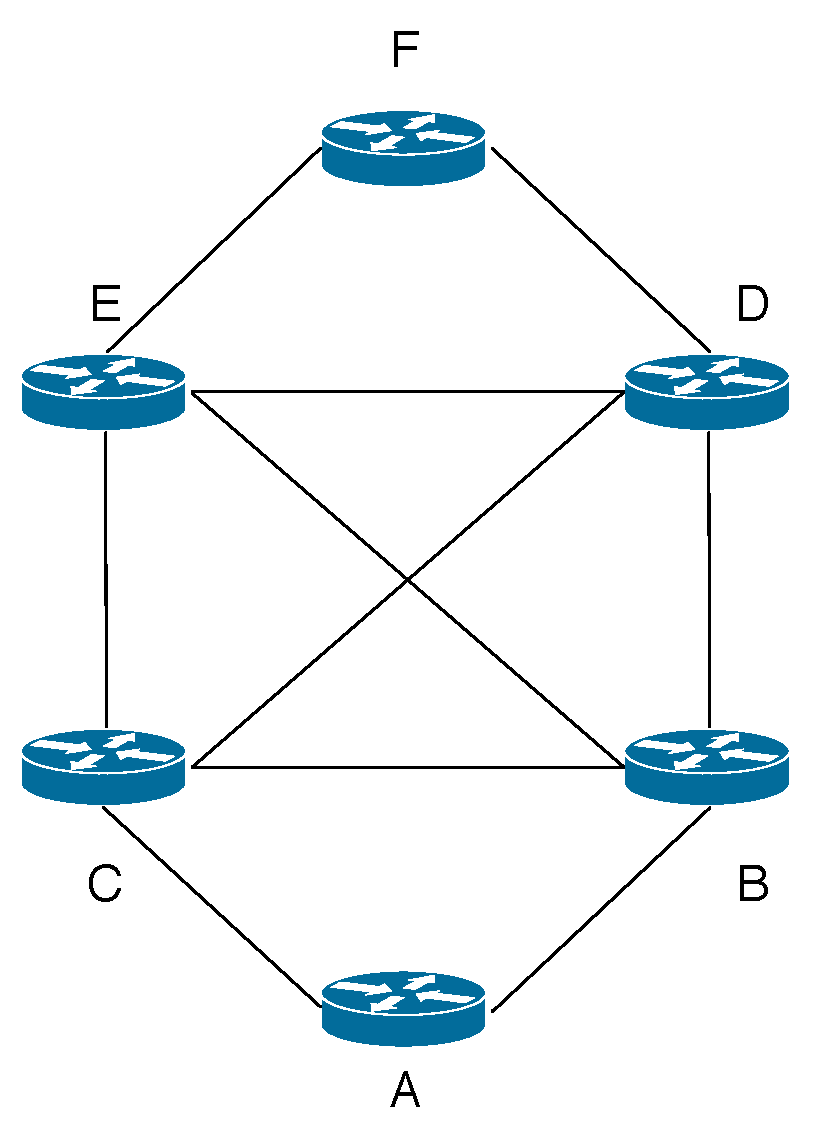
\includegraphics[scale=.75]{TestBed}
\caption{The reference topology.}
\label{fig:testbed}
\end{figure}

 
\subsection{The Classical - MultiRoute}

The classical implementation of MultiRoute is based on a single bit representation of congestion, which allows it to leverage local and remote congestion information. It is based on an approach similar as the one used in Random Early Marking \cite{REM} (REM). 

\subsubsection{Protocol Detail}

As stated above, MR is modeled on REM. Each router probabilistically marks a link as congested, this congestion information is then sent to neighboring routers allowing them to modify their route selection algorithm. Links are marked congested following an exponential measure of the link congestion (ie. the transfer function), doing so ensures that the marking probability is also exponential for the path congestion measure.

Achieving the behavior described above requires that each router to obtains both the
available paths for routing and their associated statistics. Conveniently, the
Path Discovery algorithm described in Section \ref{sect:MRPC} delivers
MultiRoute (MR) \cite{MR} with a set of valid multipaths available for
routing. Based on this set of links, MR builds a preliminary routing table
indicating the set of paths available for each destination. This, then, allows
MR to construct the \textit{Routing Mask} (shown in Figure \ref{fig:RM})
representing the structure used by the congestion updates. The local and remote
congestion information received from neighboring routers allows the current
router to build the final routing table which only contains the best (in terms
of congestion) next-hop to all destinations. The algorithm by which this table
is built is detailed in Section \ref{sect:MRAlgo}. 

The update message received from a neighboring routers is compared to the
\textit{Routing Mask} obtained initially from that same router. By aligning the
\textit{Routing Mask} and the update message, as shown in Figure
\ref{fig:RMCompare}, it is clear to the current router how to interpret the
update message and therefore it is evident which paths for each destination
are congested. Thereby, enabling a simple method to compute the final
routing table. 

Actually, the final routing table can be pre-computed as all the information to determine the next-hop for each destination is available before packets to these destinations arrive. Pre-calculating the final routing table is justified by the fact
that in the worst case update messages will be received at one second intervals as
this is the minimal polling interval router support for counter updates \cite{YaTG}.
Moreover, it minimizes the flow setup time as the router now only needs to
perform a lookup in the routing table to obtain the best next-hop.

\ifigure{RMCompare}{0.5}{Comparing a \textit{Routing Mask} with its an Update Vector}{fig:RMCompare}
% Build figure of comparison between remote routing mask and associated update vector. 
%	show sections which identify networks RMCompare

MultiRoute's Monitoring Protocol delivers the MR with raw statistics from the interface counters. MR then uses the transfer function shown in Equation \ref{eq:MRTF} to compute a 1-bit probabilistic marking of the router-router links, where $\Delta$ is the difference between two consecutive counter values and $\Gamma$ is the capacity of the router-router link. Finally, $\Phi$ is a scaling factor set by the network operator. Basically, the larger this factor is the more probable a link will be marked.

 \begin{equation}
P[Link~is~congested] = 1 - \Phi^{-\frac{\Delta}{\Gamma}}
\label{eq:MRTF}
\end{equation}

As the link utilization ($\rho = \frac{\Delta}{\Gamma}$) increases, the
probability to mark the link increases exponentially, as shown in Figure
\ref{fig:MRTF}, where the dotted lines show the curve for different values of $\Phi$. The 1-bit marking is derived by random variable who value is compared to the output of the transfer function, if the random variable is smaller than the output of the function then the linked is marked as congested. The rational behind this is that we want to rapidly mark a link
as congested in order to shift traffic from it as early as possible. 

\begin{figure}[htbp!]
\begin{center}

\begin{tikzpicture}[scale=6.0, domain=0:1]
    \draw[very thin,color=gray,step=0.5cm] (-0.1,-0.1) grid (1.2,1.2);
    \draw[->] (-0.2,0) -- (1.2,0) node[below = 28pt, left=3pt] {$\rho = Link~Utilization$};
    \draw[->] (0,-0.2) -- (0,1.2) node[left = 28pt, below=5pt] {$\rotatebox{90}{Prob. to set congestion}$};
    \foreach \x/\xtext in {1/1}
      \draw[shift={(\x,0)}] (0pt,2pt) -- (0pt,-2pt) node[below] {$\xtext$};
    \foreach \y/\ytext in {1/1}
    \draw[shift={(0,\y)}] (2pt,0pt) -- (-2pt,0pt) node[left] {$\ytext$};

    \draw[color=black] plot[id=exp] function{(1 - 50**(-x))}
      node[above] {$f(\rho) = 1-\phi^{-\rho}$};

      \draw[color=black,dashed] plot[id=exp1] function{1 - 25**(-x)} ;
      \draw[color=black,dashed] plot[id=exp2] function{1 - 10**(-x)};
      \draw[color=black,dashed] plot[id=exp3] function{1 - 5**(-x)};
      \draw[color=black,dashed] plot[id=exp4] function{1 - 3**(-x)};

%     \draw[color=black] plot[id=exp2] function{4*(1 - 500**(-x/4))}
\end{tikzpicture}

\end{center}
\caption{The transfer function used in Classical MultiRoute.}
\label{fig:MRTF}
\end{figure}

Another factor that is important is the \textit{Routing Mask} length obtained
when using this transfer function with the classical implementation of
MultiRoute. Trivially, the \textit{Routing Mask} length, given in bits, is shown
in Equation \ref{eq:MRRMLength}. 

\begin{eqnarray}
 RM~Length &=& (N-1) + N\displaystyle\sum\limits_{i=1}^N \frac{C_{i}}{N} \nonumber \\
&=& (N - 1) + N\bar{C} \nonumber \\ 
&=& N(1 + \bar{C}) - 1
\label{eq:MRRMLength}
\end{eqnarray}

Equation \ref{eq:MRRMLength} gives the derivation of \textit{Routing Masks}
where $N$ is the number of networks, $C_{i}$ is the number of uplinks per
destination. It is difficult, if not impossible, to predict the $C_i$ values as
they are linked to the topology therefore we define $\bar{C}$ as the average
number of uplinks per destination which is equal to the sum of $C_{i}$ divided
by $N$. The first term, $(N-1)$, represents the number of separator bits in
terms of number of networks and the second term represents the number of bits
required to represent the congestion per destination. Based on this equation we
have the 3D plot in Figure \ref{fig:MRRM3D} of the length of the \textit{Routing
Mask} as a function of the average number of uplinks and the number of networks.

\ifigure{RMLength}{0.5}{\textit{Routing Mask} Length as a function of $N$ and
$C$.}{fig:MRRM3D}


\subsubsection{Features and Limitations}

MR provides an extremely lightweight mechanism to represent congestion within a
multipath network. The crucial information describing which link to which
destination is congested is maintained by the Update Messages relying on the
\textit{Routing Masks}. Therefore, rather than aggregating congestion
information at each router, MR provides congestion information for each
router-router link and represents them clearly to all routers in the network
using a single bit. Due to the use of only a single bit to represent congestion,
MR is best suited for networks in which flows are long-lived and each flow
consumes the entire bandwidth offered by the router-router link. 

Moreover, MR uses a minimal amount of processing power at flow setup time as it
pre-computes the best next-hop for each destination. The selection algorithm
which builds the final routing table requires itself few resources. First, it
does not create any extra data structures, thereby requiring no extra memory.
Second, it is essentially a comparison algorithm and the elements of the
comparison are delivered in a simple form (Update Message). Therefore the
computation is
straightforward as shown in Section \ref{appdx:MR}. Overall, the  protocol
maintains just one extra table more than legacy protocols (such as
Shortest Path protocols). All protocols maintain a
routing table which contains the next-hop to any destination, MR also maintains the
preliminary routing table which contains all the possible paths to any
destination obtained from the path construction component.

As MR functions by receiving signals from neighboring routers, it is clear that
the main problem is the signal propagation time. Due to the congestion on the
paths, signals may either be delayed significantly or in the worst case, lost.
MMP, which is responsible for delivering the monitoring messages, does not
verify if messages arrive at their destination (thereby behaving like UDP). As
congestion increases, the probability to delay or lose packets increases
significantly but as MR monitoring messages only contain an Update Message
plus an MMP packet header they are very small (typically less than 200 bits as
shown in Figure \ref{fig:MRRM3D}). Therefore, the risk of delaying or losing
packets is mitigated by the size of the packets themselves. 

Another limitation is given by the \textit{Routing Mask} length itself. It is
known that the Maximum Transmission Unit (MTU) for an IPv4 path is 576 bytes,
and the MMP protocol does not support fragmentation\footnote{Moreover,
fragmentation is nowadays considered harmful \cite{FragBad}}. By setting \textit{RM Length} to
$576 * 8$ bits in Equation \ref{eq:MRRMLength}, we can see that there is an
inverse relationship between the number of networks and the average number of
uplinks per destination as shown in Figure \ref{fig:LenLim}. Considering that MR
is an interior-gateway routing protocol, an unreasonably large number of networks
and/or parallel uplinks would be required to exceed the MTU limit. 


 \begin{figure}[htbp!]
 \begin{center}
 
 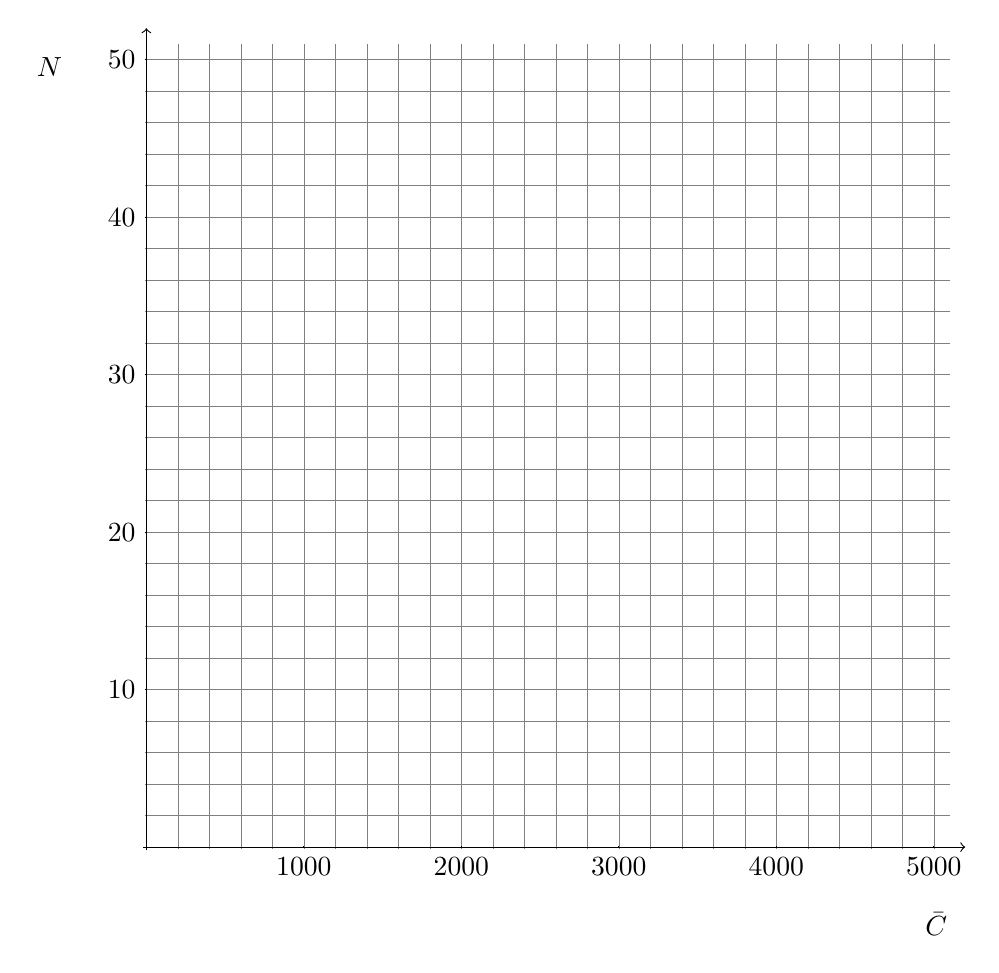
\begin{tikzpicture}[scale=0.2, domain=0:46]
     \draw[very thin,color=gray,step=2] (-0.1,-0.1) grid (51,51);
     \draw[->] (-0.2,0) -- (52,0) node[below = 28pt, left=3pt] {$\bar{C}$};
     \draw[->] (0,-0.2) -- (0,52) node[left = 35pt, below=7pt] {$N$};
     \foreach \x/\xtext in {10/1000, 20/2000, 30/3000, 40/4000, 50/5000}
       \draw[shift={(\x,0)}] (0pt,2pt) -- (0pt,-2pt) node[below] {$\xtext$};
     \foreach \y/\ytext in {10/10, 20/20, 30/30, 40/40, 50/50}
     \draw[shift={(0,\y)}] (2pt,0pt) -- (-2pt,0pt) node[left] {$\ytext$};
 
     \draw[color=black] plot[id=line] function{(4608/(1+x))/100};
 
 %     \draw[color=black] plot[id=exp2] function{4*(1 - 500**(-x/4))}
 \end{tikzpicture}
 
 \end{center}
 \caption{Plot of the \textit{Routing Mask} Limitation}
 \label{fig:LenLim}
 \end{figure}
% PLOT 577*8/(1+C)!!! IN TKZ

  % Signal propagation time
  % Routing Mask length.
  % return path is itself extremely congested however this is mitigated by size.
      % as packet loss probability increases with congestion direct from queue.
% marks links as congested too early

\subsubsection{Routing Algorithm}
\label{sect:MRAlgo}

The Routing Algorithm in MR, given all the congestion indications, constructs the best (or least congested) next-hop based on the set of available paths obtained from the preliminary table. The pseudocode is given in Section \ref{appdx:MR}. The Routing Algorithm considers both local and remote congestion information and we distinguish three cases in which the algorithm operates:

\begin{itemize}
 \item \textit{Case I - All local paths uncongested.} In this case, we consider the remote congestion statistics relevant to the destination under consideration. If there are multiple local paths available, for each potential next hop the number of uncongested paths are counted. The local path associated to the next hop with the least congested paths is selected, thereby maximizing the probability that the traffic will be forwarded unhindered. On the other hand, if all the remote congestion counts are equal or if there are multiple candidates, the shortest path is selected.
 \item \textit{Case II - Some local paths are congested while others are not.} Here we first consider the uncongested local paths in ascending path lengths. Then the associated remote paths are inspected, if one is found that is not congested then it is selected as a next hop. Otherwise, the shortest path is selected. This case will attempt to fill available and uncongested paths, thereby increasing the overall throughput of the network.
 \item \textit{Case III - All local paths are congested.} In this last case, we perform a search which is similar to the first case. The idea being that we want to find a path that is well suited to accommodating more traffic. If none is found, we select the shortest path again.
\end{itemize}

It is clear from the outline of the algorithm that in the worst case the algorithm will always select the shortest path. Moreover, the algorithm favors the shortest path first, and only once this path is considered congested does the algorithm switch to an alternative path. This approach guarantees that the algorithm cannot perform worse in terms of throughput than the current shortest path algorithms.

Consider now the network shown in Figure \ref{fig:testbed} and the associated routing table given in Table \ref{tab:matrix}, and multiple flows originating from the network under router F with destination network at router A. For the purpose of this example, let us assume that the flow's inter-arrival time at the source router is greater than the update interval at neighboring routers\footnote{In practical terms, these routers poll their local statistics at one second intervals, therefore the update time is one second plus the update message transmission time.}. We also assume that each flow is long lived and immediately consumes the entire bandwidth of the path it utilizes. There are four paths between networks F and A, namely F-D-B-A (1), F-D-C-A (2), F-E-C-A (3), and F-E-B-A (4), path (1) is considered to be the shortest followed by path (2) and so on. As there are only two distinct paths we can expect to double the network throughput with respect to a shortest path algorithm.

When the first flow arrives, it is bound to path (1) as this path is considered to be the shortest, and due to Case I, this then causes an update from the routers F, D, and B indicating that their links are congested. When the next flow arrives, the decision is taken by Case II of the algorithm, and therefore the algorithm will consider the paths with next hop E as this link is not congested. The path (4) is excluded, because the link between B and A is congested due to the first flow. Therefore the second flow is bound to path (3). Finally, for each subsequent flow, Case III of the algorithm will apply. The next two flows will be bound to paths (2) and (4) respectively, and the rest will be sent along the shortest path.

\subsection{The Organizer - StepRoute}

StepRoute \cite{SR} is a variant of MultiRoute which enables the network administrator to
define congestion classes. These classes allow for a finer control of the
congestion of the network and therefore enable for a more efficient use of the
network resources.

\subsubsection{Protocol Detail}
\label{sect:SRDetail}

StepRoute contrasts with MultiRoute by first extending the \textit{Routing Masks} to accommodate the definition of congestion classes. Second, it uses a linear transfer function rather than an exponential one in order to simplify the definition of the congestion classes. Based on a predefined value, a link is deemed to be part of one of the congestion classes. 

By classifying congestion into classes and using \textit{Routing Masks}, we are able to deliver timely information to routers while maximizing the accuracy of the delivered statistics. Each router has to define the same number of congestion classes, otherwise neighboring routers will not be able to interpret the \textit{Routing Masks} received correctly.  

 \begin{equation}
\gamma = \frac{\Delta}{\Gamma}
\label{eq:SRTF}
\end{equation}

In a similar fashion to MR, StepRoute obtains its raw statistics from MMP.
StepRoute then classifies the link into the corresponding congestion class based
on the transfer function, shown in Equation \ref{eq:SRTF}, and the congestion
classes defined in Table \ref{tab:CongClass} where the $\alpha$ values are the congestion class boundary value. As the link utilization increases
the link is classified into a higher congestion classes, thereby simplifying the
process by which the Routing Algorithm will select the next-hop, ie. favor
links in lower congestion classes.

\begin{table}[h!]
  \begin{center}
    \begin{tabular}{| c || c |}
\hline
 Class 1  & $ 0.0 < \gamma \leq \alpha_1$ \\
 Class 2  & $ \alpha_1 < \gamma \leq \alpha_2$ \\
 Class i  & $ \alpha_{i-1} < \gamma \leq \alpha_i$ \\
 Class P  & $ \alpha_{P-1} < \gamma \leq \alpha_P = 1.0$ \\
\hline
    \end{tabular}
  \end{center}
  \caption{Congestion Classification.}
\label{tab:CongClass}
\end{table}

Figure \ref{fig:SRTF} depicts the linear transfer function used in StepRoute. In
this variant of MultiRoute, it is preferable to use a linear transfer function
as we wish to distribute traffic equally amongst all the links we have at our
disposal. If an exponential transfer function had been used then links would
quickly fall into the highest congestion class and links with unused
bandwidth would not be used. 

\begin{figure}[htbp!]
\begin{center}

\begin{tikzpicture}[scale=6.0, domain=0:1]
    \draw[very thin,color=gray,step=0.5cm] (-0.1,-0.1) grid (1.2,1.2);
    \draw[->] (-0.2,0) -- (1.2,0) node[below = 28pt, left=3pt] {$\rho = Link~Utilization$};
    \draw[->] (0,-0.2) -- (0,1.2) node[left = 28pt, below=5pt] {$\rotatebox{90}{Congestion Value}$};
    \foreach \x/\xtext in {1/1}
      \draw[shift={(\x,0)}] (0pt,2pt) -- (0pt,-2pt) node[below] {$\xtext$};
    \foreach \y/\ytext in {1/1}
    \draw[shift={(0,\y)}] (2pt,0pt) -- (-2pt,0pt) node[left] {$\ytext$};

    \draw[color=black] plot[id=linear] function{(x)}
      node[above] {$f(\rho) = \rho$};

     
%     \draw[color=black] plot[id=exp2] function{4*(1 - 500**(-x/4))}
\end{tikzpicture}

\end{center}
\caption{The transfer function used in StepRoute.}
\label{fig:SRTF}
\end{figure}

Using such a classification mechanism we can simply encode the congestion class
number in the Update Message. Therefore if we would like to represent $m$
classes of congestion where $m$ can be expressed as $2^{n}$, then we only need
$n$ bits per router-router link are needed to represent all the congestion
classes. Therefore, as the number of congestion classes grows exponentially, the
space required to represent them, in the Update Message, grows linearly.
This method allows us to describe
many congestion classes while employing a lightweight, and therefore easily
distributable, representation.


%\begin{figure}
%\begin{center}
%\begin{tikzpicture}[scale=0.5, domain=0:4]
%    \draw[very thin,color=gray] (-0.1,-1.1) grid (3.9,16.9);
%    \draw[->] (-0.2,0) -- (4.2,0) node[right] {$n (bits)$};
%    \draw[->] (0,-1.2) -- (0,17) node[above] {$f(n)$};
%    \draw[color=black] plot[id=2x] function{2**x} 
%        node[right] {$f(n) = 2^{n}$};
%\end{tikzpicture} 

%\end{center}
%\caption{The number of congestion classes representable per X bits}
%\label{fig:classes-explin}
%\end{figure}

On the other hand, using multiple bits to represent the congestion class will require longer \textit{Routing Masks} as each entry for each destination in the \textit{Routing Mask} is now $n$ bits long.  We therefore have Equation \ref{eq:SRRMLength} which represents the length of the \textit{Routing Masks} in StepRoute. 

\begin{eqnarray}
 L &=& (N-1) + N\displaystyle\sum\limits_{i=1}^N \frac{nC_{i}}{N} \\
&=& (N - 1) + Nn\bar{C} \\ 
&=& N(1 + n\bar{C}) - 1
\label{eq:SRRMLength}
\end{eqnarray}

Equation \ref{eq:SRRMLength} is identical to Equation \ref{eq:MRRMLength} if we
set n, the number of bits required to represent the congestion classes, to one.
Therefore, all the other terms in Equation \ref{eq:SRRMLength} represent the
same thing as for MR.

%%%% 3d FIGURE OF ROUTING MASKS!!! FROM MATLAB!! <- NOPE!

\subsubsection{Features and Limitations}

As StepRoute is built on top of MultiRoute it inherits all the functionality that MR had, but also it also suffers from the limitations of MultiRoute. Namely, it suffers from the same problem of signal propagation time and the potential \textit{Routing Mask} length. Due to the fact, that StepRoute uses more bits in the \textit{Routing Masks} than MultiRoute, it supports less networks or less connections per destinations. In other words, the inverse relationship between number of networks and number of connections in StepRoute is steeper than in MultiRoute.

StepRoute uses slightly more memory than MultiRoute as it requires three tables. The first two are also found in MultiRoute, the third table is used to convert the raw congestion value into a congestion class. The size of this table depends entirely on the number of congestion classes and therefore it is safe to say that it contains $n-1$ entries.

StepRoute allows for a finer control of the congestion on the network. By
defining multiple congestion classes, StepRoute can represent the current level
of congestion to neighboring routers and therefore attempt to install flows onto
paths which have enough bandwidth to support the new flow. This approach leads
to much better usage of the network resources especially in the presence of
flows which do not consume the entire bandwidth of router-router links.
Typically, if the the router uplinks have a much larger capacity than the
underlying network, StepRoute will load balance this traffic much more
efficiently than MultiRoute, as flows will always consume a fraction of the
capacity of the uplink and therefore the congestion classes will describe more precisely the partial congestion present on each uplink.

%%RETHINK CONCLUSION!

\subsubsection{Routing Algorithm}

Similarly to MultiRoute, StepRoute distinguishes three cases which represent the state of the congestion local to the router. Then, based on these three cases it selects the current best next-hop from the preliminary routing table and constructs the final routing table.  The pseudocode is given in Section \ref{appdx:SR}. We should note here that the algorithm considers the lowest congestion class as already being congested and therefore attempts to avoid the potentially lightly loaded link.

\begin{itemize}
 \item \textit{Case I - All local paths uncongested.} In this case, the
algorithm only looks at the statistics received from neighboring routers.
Assuming there are multiple paths available, the router searches for the least
congested path which is simple due to the classification of the congestion
values discussed in Section \ref{sect:SRDetail}. Clearly, if the
algorithm finds a remote path with is not at all congested, it immediately
selects this path for forwarding. On the other hand, if all the remote
congestion counts are equal or if none is found, the shortest path is selected.
 \item \textit{Case II - Some local paths are congested while others are not.}
This case is slightly more complex because a local path, even if it is carrying
some traffic, may still be amongst one of the better options. This is due to
the fact that remote paths, which lay beyond a completely uncongested link, may
be completely congested. In this case, the algorithm ranks the candidate paths
by summing their local congestion with the remote congestion. The path with the
lowest congestion value is then selected. As with Case I, if there are multiple
candidates, the shortest one is selected.
 \item \textit{Case III - All local paths are completely congested.} This case
is very much similar to the first case. The idea here is to look at the
congestion values of remote routers and determine the least congested path, in
an effort to use up all the available bandwidth. Again, if multiple candidates
are found, the algorithm defaults to the shortest path.
\end{itemize}


Let us consider, as an example, the network given in Figure
\ref{fig:testbed} and its associated Table \ref{tab:matrix}, when multiple
flows enter at router F destined for network A. We also assume that each flow is
long lived  and that it immediately consumes half of the available bandwidth.
There are four paths between networks F and A, namely F-D-B-A (1), F-D-C-A (2),
F-E-C-A (3), and F-E-B-A (4), path (1) is considered to be the shortest followed
by path (2) and so on. As there are only two distinct paths we can expect to
double the network throughput with expect to a shortest path algorithm. It is
important to note that, with respect to the real implementation the routing
tables are pre-computed as statistics become available and not when a flow
arrives.

When the first flow arrives, it is bound to path (1) as this path is considered
to be the shortest, and due to Case I, this then causes an update from the
routers F, D, and B indicating that their links are partially congested. When
the next flow arrives, the decision is taken by Case II of the algorithm, and
therefore the algorithm will consider the paths with next hop E as this link is
not congested. The path (4) is excluded, because the link between B and A is
congested due to the first flow. Therefore the second flow is bound to path
(3). Upon arrival of the third flow, Case II will rank the available paths
according to the congestion level and will choose path (2) as the link between
D and C is not congested. Similarly, when the fourth flow arrives, Case II
ranks the available paths again and picks path (4). As subsequent flows arrive
at router F, Case III attempts to find available bandwidth to send the flow on
and if this is not possible it sends it onto the shortest path.


Similarly to MultiRoute, the algorithm defaults to the shortest path as well. This default is to reduce the delay experienced by the packets in the situation where no best option exists. 
  

\subsection{The Know-it-all - PathRoute}

While MultiRoute provides a link by link measure of the path congestion, PathRoute provides the actual congestion over the entire path from a given source to any destination. MultiRoute could in certain circumstances lead traffic into a congested area of the network due to a lack of knowledge of the effective distant congestion. PathRoute, by reporting entire path congestion at every router, avoids this situation and will never lead traffic into a congested area to the extent of the possible of course. 

While the previous two protocols limited themselves to distributing update
vectors to their direct neighbors only, PathRoute concatenates the information
contained in update vectors to deliver the path congestion for each router. To
achieve this objective PathRoute uses the same transfer function as MultiRoute
and also represents congestion on a single bit. The difference resides in the
fact that now the protocol analyzes the information received from its neighbors
to derive the path congestion. In order to distribute path congestion, 
PathRoute needs to know two pieces of information:

\begin{enumerate}
\item The set distances from a given router to all the other routers in the network. This will allow PathRoute to define the length of the \textit{Routing Masks} and therefore construct the initial mask which will be used to inform neighboring routers about the structure of the update messages.
\item The set of congestion information that should be concatenated at each
router and sent to neighboring ones.  A router needs to determine which part of
an update message is relevant to it, then concatenate this information and send
it to neighboring routers.
\end{enumerate} 

The first problem is solved using Diffusion Algorithms with termination
detection \cite{DijkstraTerm}. Each router initiates a computation by outputting
an Update MMP of code INIT on each of its router-router links for each destination and
keeps track of the number of messages it has sent and received. Next, when a
router receives an Update MMP with code INIT, it checks whether the packet is
destined for it, if it is then the router increments the distance counter
(contained in the packet), changes the code of the packet to NEW and replies to
the source over the shortest path. Otherwise, the counter is incremented and the packet is forwarded to the
destination, if the current router has multiple paths to the destination it
duplicates the packet and sends it down each of the uplinks for that
destination. Then, if a router encounters an MMP with NEW code, it checks
whether its number of sent and received messages is equal, if yes it sends the
reply towards the source along the shortest path otherwise it simply stores it.
Doing so, guarantees that if router sends a reply it is either the destination
of the query or it has received as many queries as it has sent and therefore by
the time the source obtains a reply we know that the computation has terminated.
Finally, when the source receives a reply it updates its distance table. The
flowchart in Figure \ref{fig:distflow}. Once all the routers have computed their
relative distances, each router can now construct and send their \textit{Routing
Mask} to their neighbors. This process occurs at the initial state of the network and therefore we assume that no other traffic can interfere with this process. 

%%FLOW CHART DIFF COMP & figure of aggregation...
\ifigure{DistFlow}{0.4}{Flowgraph of the distance diffusion computation.}{fig:distflow}

The second issue can be divided into two sub-problems. First, knowing that each
entry for a destination in the Update Message contains the entire path
congestion to that destination, the protocol must first know where to insert its
local congestion information. Second, when receiving an update message the
router must identify the parts of the update message which are of interest to
it, ie. the parts which describe the congestion to one or more of its
destinations.

The first sub-problem can be solved quite easily. Knowing the distance and the
number of uplinks for any destination, given by the distance table and the
preliminary routing table respectively, the router can easily identify the first
bit of a path description which will be the congestion value for its local
uplink.  The following sub-problem relies on the structure of the
\textit{Routing Mask}. When a router receives an update message, it first
determines if the port on which the message is received is used for any
destination and if so, is the distance to the destination on this port greater
than one? Then by comparing the message with the \textit{Routing Mask}, just
like in MultiRoute or StepRoute, it determines which parts of the update
message contain information about one or more of its destinations. The router
can simply copy the interesting parts of the update message into its own update
message, by concatenating the local congestion on the uplink with information
received in the update message from the neighbor. This new update message is
then propagated to the neighbors which therefore distributes the congestion
information around the network and enables routers to build their view of the
path congestion. This process is referred to as the aggregation step of
PathRoute. 

The major side-effect of representing the entire path congestion within the update messages is that their length increases significantly. While this is intuitively trivial, it is not so clear analytically since it is impossible to formalize the path length as it is intimately coupled to the network topology. Therefore  we can only predict the message size by specifying an average path length, $\bar{P}$, as shown in Equation \ref{eq:PRRMLength}.

\begin{eqnarray}
 L &=& (N-1) + N\displaystyle\sum\limits_{i=1}^{N} P\frac{C_{i}}{N} \\
&=& (N - 1) + N\bar{P}\bar{C} \\ 
&=& N(1 + \bar{P}\bar{C}) - 1
\label{eq:PRRMLength}
\end{eqnarray}

\subsubsection{Features and Limitations}

PathRoute delivers an extremely space and computation efficient mechanism for representing the path congestion at each router. By computing the distance from any router to another, PathRoute is able to extend its \textit{Routing Mask} with space to describe every link along the path to a destination and therefore deliver full path congestion information to every router. Finally, since each router running PathRoute knows all the information about the status of the path to the destination, the resulting routing algorithm is very simple and only requires information which is locally stored which therefore enables rapid flow installation.

By design, MultiRoute may unknowingly route traffic into congestion since it only has congestion information about its local links and its neighbors links. Therefore, if congestion lies beyond the next-hop andthe next-hop has no other option then MultiRoute may exacerbate the congestion in some areas of the network. PathRoute, on the other hand having full knowledge of path congestion, will never route traffic into congestion unless there is no other option available to it. 

Even though PathRoute provides deep information about the status of the network to each router, it requires no more memory than StepRoute. Three tables  are required, a preliminary routing table, a final routing table, and a distance table. On the other hand, initially, PathRoute requires slightly more CPU power as it must send MMP packets to compute the relative distances from one router to another.

As PathRoute is built on top of MultiRoute, it suffers from the same problems. Moreover, since update messages may be aggregated, the propagation delay for an update message is potentially multiplied by the path length. Therefore, the probability of delay or drop of the update message is also increased, but again this is mitigated by the relatively small size of these messages. 

\subsubsection{Routing Algorithm}

As each router now has all the information about the path congestion, there is no longer a need to distinguish three cases for the routing algorithm. PathRoute's routing algorithm takes the simplest form. More precisely, it simply finds the least congested path and forwards packets through the associated next-hop. As shown in \ref{appdx:PR}, the routing algorithm is straightforward and simply counts the number of links which are not congested. The path which contains the least number of congested links is selected.

Consider, once again, the network given in \ref{fig:testbed} and its associated
connectivity Table \ref{tab:matrix}, when flows originate at multiple routers in
the network. Let us also assume that each flow directly consumes the entire
bandwidth proposed by the path. We assume that the source routers are F, D, and E and a single destination
A. Therefore, the available paths are F-D-B-A (1), F-D-C-A (2), F-E-C-A (3), 
F-E-B-A (4), D-B-A (5), D-C-A (6), E-C-A (7), and E-B-A (8). 

Considering the situation described above, two flows arrive at router F. Based on PathRoute the first flow will select path (1) and the second path (2). Now, a flow arrives at router D, since path (5) has now two congested links (D-B and B-A) caused by the first flow. Router D selects path (6) which only has one congested link. The same occurs for the flow that originates at Router E and path (8) is selected.  We can see that PathRoute will attempt to use all the links of the networks before sharing full paths.
	
\subsection{Implementation Experience}

The entire MultiRoute family was designed and implemented within NOX (see
Section \ref{sect:OPFW}). NOX is a controller API for OpenFlow whose main
advantage is the exposition of a simple API  which enables the rapid
prototyping of research networking protocols. NOX introduces the concept of
components which can be viewed as black boxes computing a certain function, for
example, compute the set of shortest paths within a network. NOX components
communicate via events and direct message passing.


The design of the MultiRoute family is based on components. Each function
described the previous section is implemented with a component. The component
itself may be further segmented into various files. The code which makes up the
MultiRoute suite is highly modular. Each protocol depends on different
components. Changing these components modifies the behavior of the protocol. For
example, switching the transfer function in MultiRoute for the one which
computes congestion classes yields the StepRoute protocol. Figure
\ref{fig:MRDeps} show the dependency maps for each protocol, notice that each
protocol differs only in some of the components used. Since similar components
expose identical API or produce the same events, most of the code from one
protocol to another is re-used. This design accelerates the implementation cycle
and guarantees that the code is stable from protocol to the next. Moreover, the
implementation was almost exclusively done using Python \cite{Python} which
means that the implementation itself was simple and is easily understandable.
  
\ifigure{DepMap}{0.5}{Inheritance/Dependency graph for MultiRoute-based protocols }{fig:MRDeps}  
  
%discuss modularity of the MR suite
% change behavior by simply changing transfer function
% change routing algorithm to change next-hop selection.
% Enables switching of protocol mid flight

\section{Commodity Protocols}

The protocols detailed below were implemented to enable us to test
MultiRoute-based protocols against the protocols which are used today in
industry. Each of these protocols were implemented on our OpenFlow-enabled
testbed.

%Protocol to test against...

\subsection{Shortest Path}

Shortest Path Routing is a direct application of Dijkstra's Shortest path
algorithm \cite{DIJK}. In essence, it is a destination-based, load-insensitive
routing algorithm which is built based either on the minimum hop count or sum of
link weights. Therefore, given a destination the routing algorithm performs a
lookup in its routing table, which contains the next-hops to every destination,
and returns the next-hop of the shortest path to the requested destination.

This protocol is made to resemble OSPF \cite{OSPF} as much as possible without
having to re-implement the totality of OSPF. This is justified, as we are only
interested OSPF's routing model but not its distributed nature nor all its
extra functionality.

\subsection{Equal Cost MultiPath}

Equal Cost MultiPath (ECMP) \cite{RFC2991} is similar to Shortest Path routing in
that it is also destination-based but it differs in the fact that multiple best
paths may be used to forward packets. Therefore, as it name indicates, if the
network contains multiple shortest paths between any source-destination pair
then they are all used to forward packets.

Normally, ECMP uses a hash which is computed based on the source and
destination mac-address contained in the packets. In our case, out network
testers and machines connected to our testbed only have a limited number of mac
addresses. Therefore, to increase the diversity of the hash, we have computed
based on the source and destination port numbers which are random for every
flow. 

Section \ref{sect:HTE} derives and explains the number of disruptions to expect
when a link of an ECMP set goes offline.

\section{Theoretical Delay Model for MultiRoute-based protocols}

In this section, we will use the model detailed in Section
\ref{sect:queues} to derive a delay model for Congestion-Aware Routing
protocols. Furthermore, we also evaluate the average number of flows present
at any node in the system.

A multipath network can be seen as a system with multiple servers. Each server,
therefore would represent an uplink between nodes in the system. Routers are
then referred to as nodes. We now need to define the arrival (input) and
departure (output) models. We can safely assume that the arrival model is
Markovian since packets sent are sent from end nodes (ie. computers) are independent
and memoryless, the same goes for the output model since it only depends on the
actual packet length of the router which is constant. Therefore we can model
our first queue in the System as M/M/m queue (see \ref{sect:mmmQ}). But, as explained
in Section \ref{sect:kleindep}, we cannot simply say the same thing for any
other queue in the system as the message length and the inter-arrival times
become highly dependant. Fortunately, Kleinrock's Independence assumption
\ref{th:indep} and in particular Burke's Theorem, allow us to select a new message size at the output of each
queue independently and therefore model our entire system as independent M/M/m
queues.

Therefore, we can now say that the delay created by a certain node is the
average time spent in the system and for an M/M/m queue is given by:

\begin{equation}
 T = \frac{1}{\mu}\left(1 + \frac{P_{Q}}{m(1-\rho)}\right)
\label{eq:Delay1node} 
\end{equation}

Where $P_Q$ is given by Equation \ref{eq:MMMPQ} and $\frac{1}{\mu}$ is the
service time and $\rho = \frac{\lambda}{m\mu}$ is the utilization ratio with
$\lambda$ the arrival rate and $m$ the number of servers.

Since, we claim that each queue is independent we can state that the overall
delay in the network is simply a function of the number of hops a packet must
traverse and therefore we have:

\begin{equation}
\bar{T} = \bar{n}T
\label{eq:overallDelay} 
\end{equation}

\ifigure{delay}{0.5}{Flow delay as function of the load
($=\frac{\lambda}{m\mu}$) and number of servers.}{fig:delay}

Figure \ref{fig:delay} shows that as the arrival rate increases the overall
load on the system increases and eventually leads to $\infty$ which is to be
expected because the expression for delay is dominated by $1 - \rho$

Another interesting quantity is the number of clients (ie. flows) that are
present at any queue. This quantity will allow us to determine the expected
disruption should a queue become unavailable for some reason.

\begin{equation}
 \bar{N} = m\rho + \frac{\rho P_{Q}}{1-\rho}
\label{eq:disruptions} 
\end{equation}


Since Equation \ref{eq:disruptions} is also dominated by $1 -\rho$, we would
have the same behavior than in Figure \ref{fig:delay}. Namely, as the system
load increases the number of flows in queue will increase as well. Figure \ref{fig:queuers} shows the number of flows waiting at each queue. We can see that as the arrival rate increases, the number of flows in the queue increases significantly. This value can also be seen as the number of flows that would be disrupted if an uplink where to go offline, thus giving us an approximation on the number of communications that would need to be re-established should there be a problem. We should note that if we pick $m=1$, then we have a model for a single path system. We can see that in such a system the delay increases significantly than in multipath systems.

\ifigure{queuers}{0.25}{Number of flows in each queue}{fig:queuers}

\section{Summary}

%Your final comment: "this seems like it missed a bit. OK, time I got here I had forgotten where it started but if I look back to the intro you talk about RFC xyz which never gets another mention. Also if the IS where you mean to end then what was the value of what you just described? Latency increases with load...nothing new there. More flows per queue as the load goes up, hmm, I don' follow, seems to me its a question of how many flows AND what their relative weights are and assuming I'm wrong, as usual then what is the conclusion: the more traffic you have the more you are fucked when one route shuts down? That's not exactly rocket science is it?  "

%You are right, I completely skipped the summary, probably cos I got bored... The point of all this is to say that while nothing super new occurs when you use multipaths, you still get more delay as the load increases, queues get more and more full and so on, but all this happens later that in the single path model. More importantly this happens later even if you coarse route (as in route by flow and not packet by packet). In itself, this a nice discovery because it means that if we route flow by flow we can still expect significant gains over single path techniques.

In this section, we have described three protocols by using the outline given in RFC 1264 \cite{RFC1264} then we gave several theoretical predictions which, while not fully accurate, provide us with an idea  of the performance we can expect of our protocols. 

The first protocol, MultiRoute, describes congestion as a single bit. While the second, StepRoute, defines congestion classes. Finally the third protocol, provides a congestion measure for the entire path from source to destination.

Using multipaths does not change the rules of the game in networks, by this we mean that the latency still increases as the load on the network increases and queues still get more and more full as the load increases. That said, all these phenomena happen when the load is higher than in the single path settings. More importantly, we also see that even though each of our protocols routes flow rather than individual packets, we can still expect a significant increase in performance while not optimal it is still quite a desirable increase over single path routing.  

%Based on previous chapter. Plot explain derivation and plot theoretical delay
% and number of flows at each node (if it makes sense).


